\documentclass{article}
\usepackage[utf8]{inputenc}
\usepackage[OT1]{fontenc}
\usepackage[french]{babel}
\usepackage{amsmath}
\usepackage{graphicx}
\usepackage[colorlinks=true, allcolors=blue]{hyperref}
\usepackage[section]{placeins}
\usepackage{listings}
\usepackage{array}
\title{Outils libres côté client}
\author{BOFFI Aurélien & SCHWARTZ Nicolas}

\begin{document}
\maketitle
\tableofcontents
\newpage

\section{TP1 - Efficacité de l'environnement}

\subsection{}

\begin{table}[h]
\centering
\begin{tabular}{l|r}

Description & Raccourci \\\hline
Discord changer de serveur  & CTRL + tab \\
\hline
Brave changer d'onglet   & CTRL + tab \\
\hline
Brave nouvel onglet   & CTRL + t \\
\hline
Brave nouvelle fenetre  & CTRL + n \\
\hline
Terminator diviser écran verticalement   & CTRL + SHIFT + e \\
\hline
Terminator diviser écran horizontalement   & CTRL + SHIFT + o \\
\hline

\end{tabular}
\caption{\label{tab:widgets}Raccourcis.}
\end{table}


\subsection{}

Le site que nous avons trouvé est le site \href{https://10fastfingers.com/typing-test/french}{\emph{Fastfingers}} qui est assez connu.

\begin{figure}[h]
\centering
    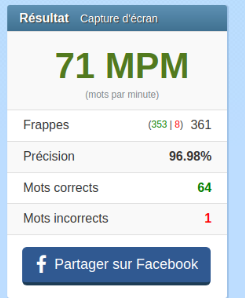
\includegraphics[height=0.7\columnwidth]{screen/Fastfingers.png}
    \caption{\label{fig:frog}Exemple d'un score du site.}
\end{figure}
\FloatBarrier

\subsection{}
\begin{itemize}
    \item Paramétrer Vim comme éditeur par défaut :
    \begin{itemize}
        \item sudo update-alternatives --config editor
    \end{itemize}
    On choisis ensuite le numéro de Vim et on confirme :
    \begin{figure}
\centering
    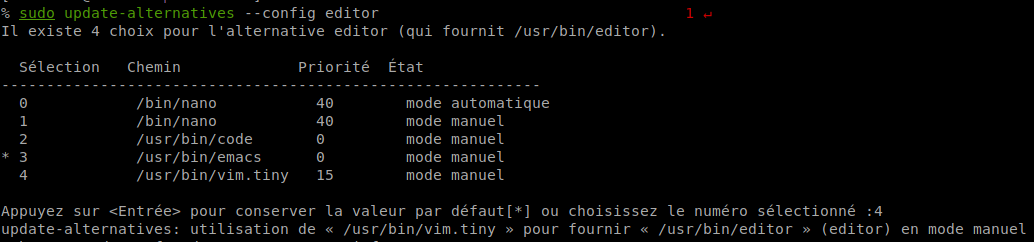
\includegraphics[width=\textwidth]{screen/Exo1-3.png}
    \caption{\label{fig:frog}Choisir son éditeur}
\end{figure}
\end{itemize}
\subsection{}
L'history peut devoiler l'emplacement de fichier sensible, il est donc important de bien le configurer.
Afin d'eviter les trés nombreux ls et cd il faut ajouter :
Dans le ~/.bashrc : HISTIGNORE="ls:cd:history"\\

\subsection{}
Pour la commande mkcd :
Dans le fichier ~/.bashrc ajouter :
\begin{lstlisting}
    function mkcd() { mkdir -p "$@" && cd "$_"; }
    alias mkcd="mkcd"\
\end{lstlisting}
Pour le script git emergency, voici le code :
\begin{lstlisting}
    !#/bin/bash
    gitemergency () {
	git add .
	git commit -m "commit d'urgence" $1
	git push
    }
    \end{lstlisting}
\subsection{}
\begin{itemize}
    \item Créer un script vide backup.sh.
    \item Ajouter le script dans /etc/bash\_completion :
    \begin{lstlisting}
    !#/bin/bash
    _backup() {
    local cur prev opts

    cur="${COMP_WORDS[COMP_CWORD]}"
    prev="${COMP_WORDS[COMP_CWORD-1]}"

    local files=("${cur}"*)

    case $COMP_CWORD in
        1) opts=`getent passwd | cut -d: -f1`;;
        2) opts="now tonight tomorrow";;
        3) opts="${files[@]}";;
        *);;
    esac

    COMPREPLY=()
    COMPREPLY=( $(compgen -W "$opts" -- ${cur}) )
    return 0
    }
    complete -o nospace -F _backup backup
    \end{lstlisting}
\end{itemize}

\subsection{}

\begin{itemize}
\item Pour ajouter le plugin vagrant prompt nous devont nous rendre dans le fichier de notre theme.
\item Les themes sont dans le dossier ~/.oh-my-zsh/themes.
\item Une fois dedans nous devons rajouter les lignes suivantes :

\begin{figure}[h]
    \centering
    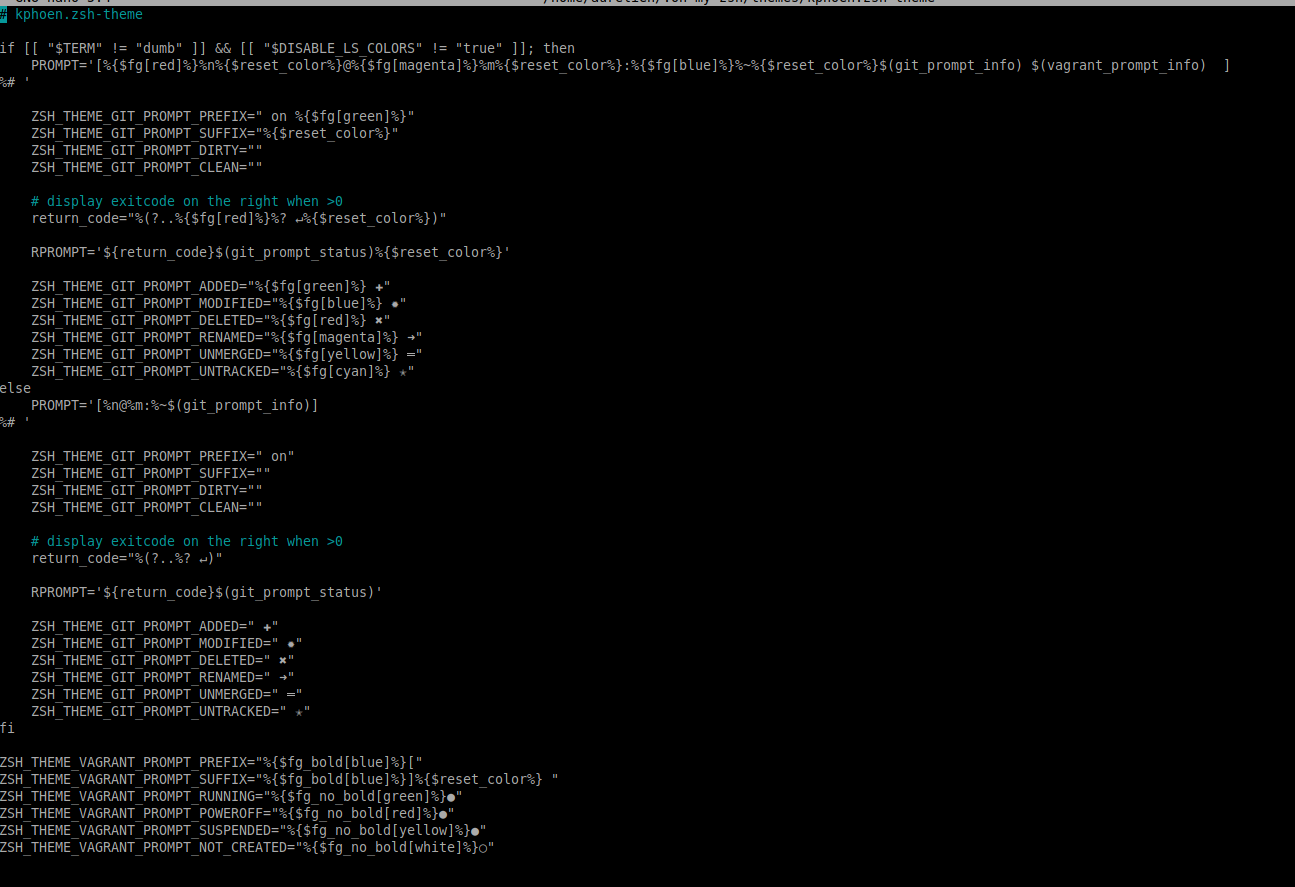
\includegraphics[width=0.7\columnwidth]{screen/1_7.png}
    \caption{\label{fig:frog}Config du theme}
    \end{figure}

\end{itemize}

\subsection{}
\begin{itemize}
\item Code à ajouter dans le fichier ~/.zhsrc
\begin{lstlisting}
double-up-history() {
         apache=$(service --status-all | grep apache2| cut -c4)
         echo $apache
         if [[ $apache == "+" ]]
         then
                echo "apache va se stop"
                sudo service apache2 stop
         else
                echo " apache va se lancer"
                sudo service apache2 start
         fi
}

zle -N double-up-history
bindkey "\C-A" double-up-history
\end{lstlisting}
\end{itemize}

\subsection{}

\begin{itemize}
    \item Terminaux testé :Terminator, kitty, coolretroterminal
    \item Terminator : plusieurs onglets ouverts assez facilement + performanant
    \item Kitty : rapide
    \item CoolRetroTerminal : difficile a utiliser en raison de son interface
\end{itemize}
\newpage

\section{TP2 - SSH}
\subsection{}
\begin{itemize}
    \item ssh alice@192.168.56.3
    \item ssh carole@192.168.56.3
    \item ssh bob@192.168.56.3
\end{itemize}
Les history sont vides car c'est la première fois que les machines sont utilisés.

\subsection{}

\begin{itemize}
    \item ssh-keygen
    \item ssh-copy-id alice@192.168.56.3
\end{itemize}
Pour déposer manuellement : 
\begin{itemize}
    \item cat /vagrant/id\_rsa.pub >> ~/.ssh/authorized\_keys 
\end{itemize}

\subsection{}

Ajout de l'host bc :
\begin{itemize}
\item
\begin{lstlisting}
Host bc
   Hostname 192.168.56.3
   User bob
\end{lstlisting}
\end{itemize}


\begin{figure}[h]
\centering
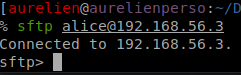
\includegraphics[width=0.7\columnwidth]{screen/ssh3.png}
\caption{\label{fig:frog}SFTP}
\end{figure}

\subsection{}
\begin{itemize}
    \item Commande : 
\begin{lstlisting}
ssh -L 8000:srv.local:80 alice@cli.local 
\end{lstlisting}
\end{itemize}

\subsection{}
\begin{itemize}
    \item Sur notre machine : ssh -D 9000 alice@cli.local
    \item Editer le fichier /etc/tsocks.conf
    \item Commenter les lignes suivantes et modifier la valeur de server\_port :
\begin{lstlisting}
#local = 192.168.0.0/255.255.255.0
#local = 10.0.0.0/255.0.0.0
server_port = 9000

\end{lstlisting}
\end{itemize}

\subsection{}
\begin{itemize}
    \item ssh bc
    \item sudo apt-get install x11-apps
    \item apt install xauth
    \item \#ForwardX11 yes
    \item ssh -X 192.168.56.3
    \item xeyes
\end{itemize}
\subsection{}
\begin{itemize}
    \item Dans ~/.ssh/config :
\begin{lstlisting}
Host srv
  Hostname 192.168.56.3
  User alice
  ProxyJump cli
#Pour ProxyCommand
 ProxyCommand ssh cli -W%h:%p
\end{lstlisting}
\end{itemize}

\newpage

\section{TP3 - GIT}

\subsection{}
\begin{itemize}
    \item git init pour créer le dossier local
    \item git add Vagrantfile pour ajouter le fichier
    \item Des fichiers sont non suivis il faut utiliser git add pour les ajouter
\end{itemize}

\begin{figure}[h]
\centering
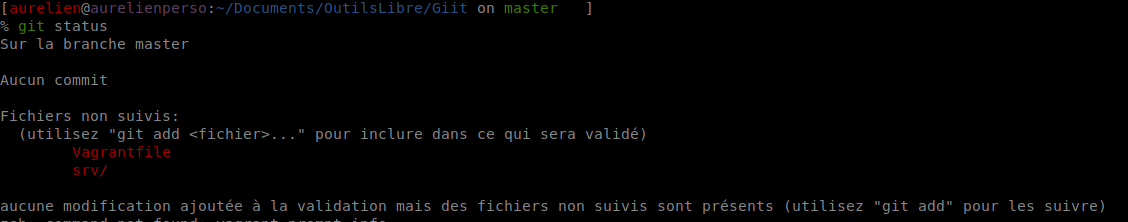
\includegraphics[width=\textwidth]{screen/git1.png}
\caption{\label{fig:frog}Status du début.}
\end{figure}

\begin{figure}[h]
\centering
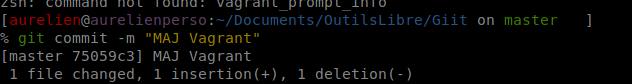
\includegraphics[width=0.7\columnwidth]{screen/git2.png}
\caption{\label{fig:frog}Le commit.}
\end{figure}

\subsection{}

\begin{itemize}
    \item git checkout -b branche
\end{itemize}

\begin{figure}[h]
\centering
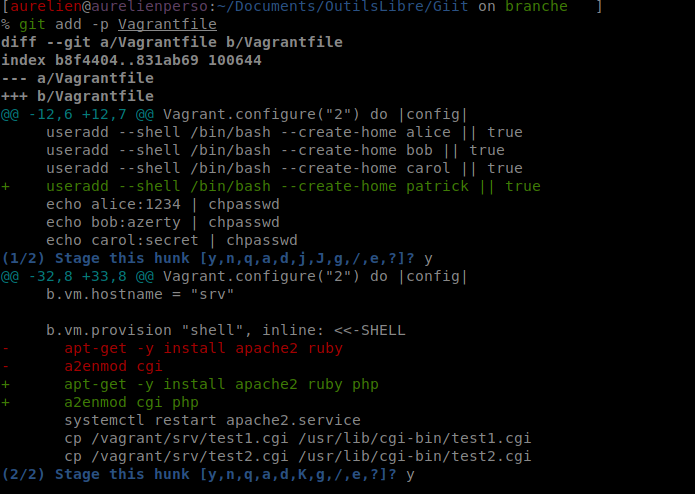
\includegraphics[width=0.7\columnwidth]{screen/git2_1.png}
\caption{\label{fig:frog}Ajout Patrick et PHP}
\end{figure}

\begin{figure}[h]
\centering
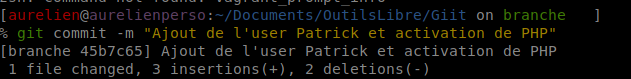
\includegraphics[width=1\columnwidth]{screen/git2_2.png}
\caption{\label{fig:frog}Le commit.}
\end{figure}

\begin{figure}[h]
\centering
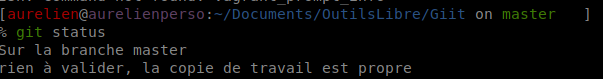
\includegraphics[width=0.7\columnwidth]{screen/git2_3.png}
\caption{\label{fig:frog}Tout va bien sur master.}
\end{figure}

\begin{figure}[h]
\centering
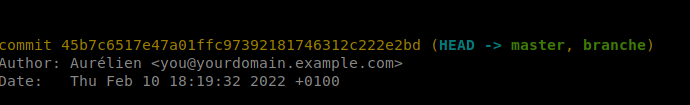
\includegraphics[width=0.7\columnwidth]{screen/git2_4.png}
\caption{\label{fig:frog}Commit bien présent.}
\end{figure}

\begin{figure}[h]
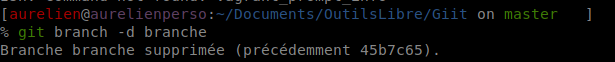
\includegraphics[width=0.7\columnwidth]{screen/git2_5.png}
\caption{\label{fig:frog}Branche supprimé.}
\end{figure}

\subsection{}

\begin{figure}[h]
\centering
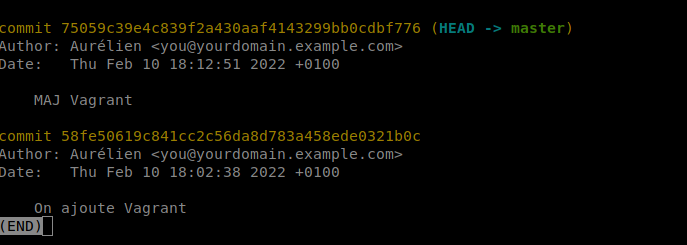
\includegraphics[width=0.7\columnwidth]{screen/git3.png}
\caption{\label{fig:frog}Commit bien présent.}
\end{figure}

\begin{figure}[h]
\centering
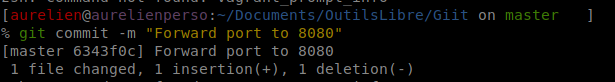
\includegraphics[width=0.7\columnwidth]{screen/git3_1.png}
\caption{\label{fig:frog}Commit ok}
\end{figure}

\begin{figure}[h]
\centering
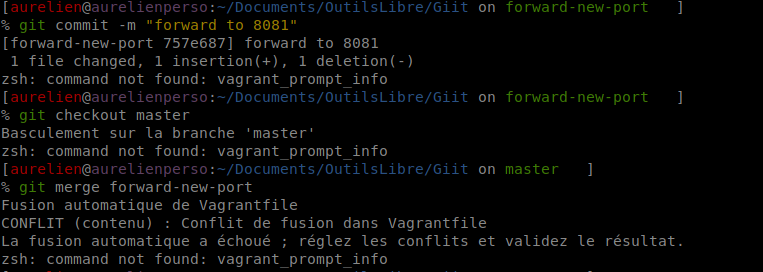
\includegraphics[width=0.7\columnwidth]{screen/git3_2.png}
\caption{\label{fig:frog}le conflit.}
\end{figure}

\begin{figure}[h]
\centering
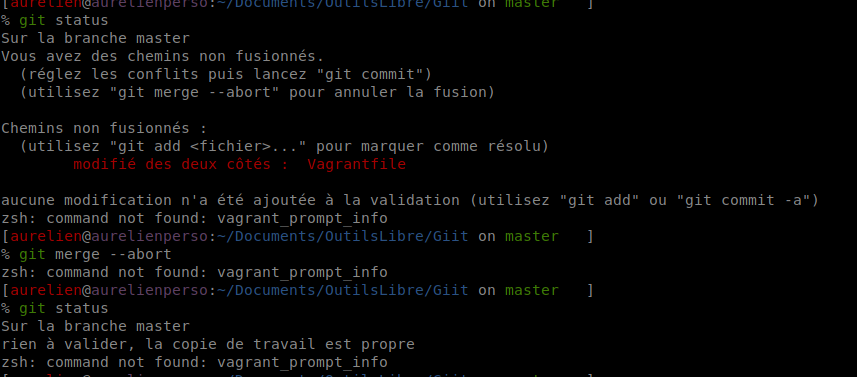
\includegraphics[width=0.7\columnwidth]{screen/git3_3.png}
\caption{\label{fig:frog}le conflit.}
\end{figure}

\begin{figure}[h]
\centering
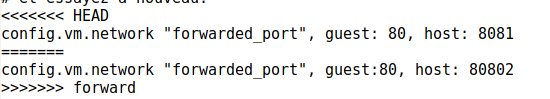
\includegraphics[width=0.7\columnwidth]{screen/git3_4.png}
\caption{\label{fig:frog}Résolution.}
\end{figure}




\end{document}